% Refactored Chapter 6: Benchmarks
% Text is unchanged; float placements improved with [htbp] specifiers and \FloatBarrier
\chapter{Benchmarks}

In this chapter, we first present performance evaluations in terms of both space and query efficiency. We then compare our method to alternative compressed graph representations and popular graph databases.

\section{Experimental Setup}

All experiments were run inside a virtual machine configured with an Intel Xeon Gold 6348 CPU (4 cores at 2.60 GHz), 62 GB of RAM, and 1 TB of storage. The VM was hosted on a Microsoft Hyper-V system and ran Ubuntu 22.04.4 LTS. While this setup provides sufficient computational resources for our evaluation, we observed that a standard 2020 consumer laptop delivered up to 2× faster performance on the same benchmarks, underscoring the impact of virtualization. Therefore, the absolute time values should be taken with a grain of salt, focusing instead on relative performance comparisons between our Compressed Graph Database and competing approaches.

We implemented the Compressed Graph Database described in previous chapters in C++, using the \verb|sdsl-lite| library for bit-packing, rank-select bitvectors, Elias-Fano encoding, and FM-index data structures. For LogGraph and CGraphIndex, we used implementations provided by their respective authors. Given that their code was not working out of the box, we manually applied minor fixes to resolve compilation errors and ensure correct functionality. Instead, we implemented CSR ourselves from scratch, again relying on the \verb|sdsl-lite| library for internal structures. Finally, we used ArangoDB 3.12.0-2 and Neo4j 2025.02.0.

In the following sections, space measurements reflect the exact on-disk size of each database. Since our compressed structures support direct querying without decompression, the memory footprint matches disk usage. The sole exception is the parent adjacency lists, which are not explicitly stored on disk because we reconstruct them easily at load time.

Additionally, we normalize all time measurements by the number of nodes retrieved, thus ensuring a fair and consistent comparison across queries of varying result size.
\FloatBarrier

\section{Overall Performance}

Table~\ref{tab:results} summarizes the space and time performance of our approach on the five datasets. The columns show space usage in MB, single-hop and two-hop neighbor query times in nanoseconds per neighbor, fixed-size property throughput in MB/s and variable-size property retrieval times in KB/s, and database build and load times in seconds. Build time refers to the process of constructing the compressed database from scratch, while load time represents the process of resuming the pre-built structures from disk. Although build times are not instantaneous, this aligns well with our assumption of static or slightly dynamic datasets where construction occurs infrequently. Furthermore, both build and load procedures could benefit from parallelization, which we did not implement in this work.

\begin{table}[htbp]
\centering
\tiny
\caption{Space and query-time performance results.}
\label{tab:results}
\begin{tabularx}{\textwidth}{lrrrrrrr}
\toprule
Dataset & Space (MB) & 1-hop (ns) & 2-hop (ns) & Fixed-size (MB/s) & Var-size (MB/s) & Build (s) & Load (s) \\
\midrule
amazon   & 177.7 &  38.1 &  10.5 & 27.3 & 0.0074 & 234.5 & 0.5 \\
dblp     & 563.9 & 122.9 & 118.9 & 25.2 & 0.0287 & 1060.0 & 12.5 \\
mag      &  27.5 &  31.9 &  18.8 & 35.5 & 0.0212 & 343.5 & 3.5 \\
patents  & 192.6 &  43.7 &  38.8 & 38.8 & 0.0132 & 194.1 & 7.3 \\
prime\footnote{The prime dataset contains no variable-size properties.}
         &  13.1 &   9.3 &   4.7 & 38.3 & -- & 5.2 & 0.3 \\
\bottomrule
\end{tabularx}
\end{table}
\FloatBarrier

We further analyzed the space usage by measuring each database component separately. Figure~\ref{fig:space_breakdown} shows how variable-size properties dominate the space usage in datasets such as \verb^amazon^, \verb^dblp^, and \verb^mag^. This is mainly due to the presence of numerous text-heavy properties, such as extensive product reviews in \verb^amazon^ or long article abstracts in \verb^dblp^ and \verb^mag^. On the other hand, datasets such as \verb^patents^ and \verb^prime^ contain mostly fixed-size properties, and this characteristic naturally influences their space distributions. Finally, we observe that the notable portion of storage required by the NodeID mapping in the \verb^dblp^ dataset is because the DBLP graph is extremely sparse but contains many nodes (around $15$M). Due to this characteristic, the NodeID mapping becomes inherently less compact.
\begin{figure}[htbp]
  \centering
  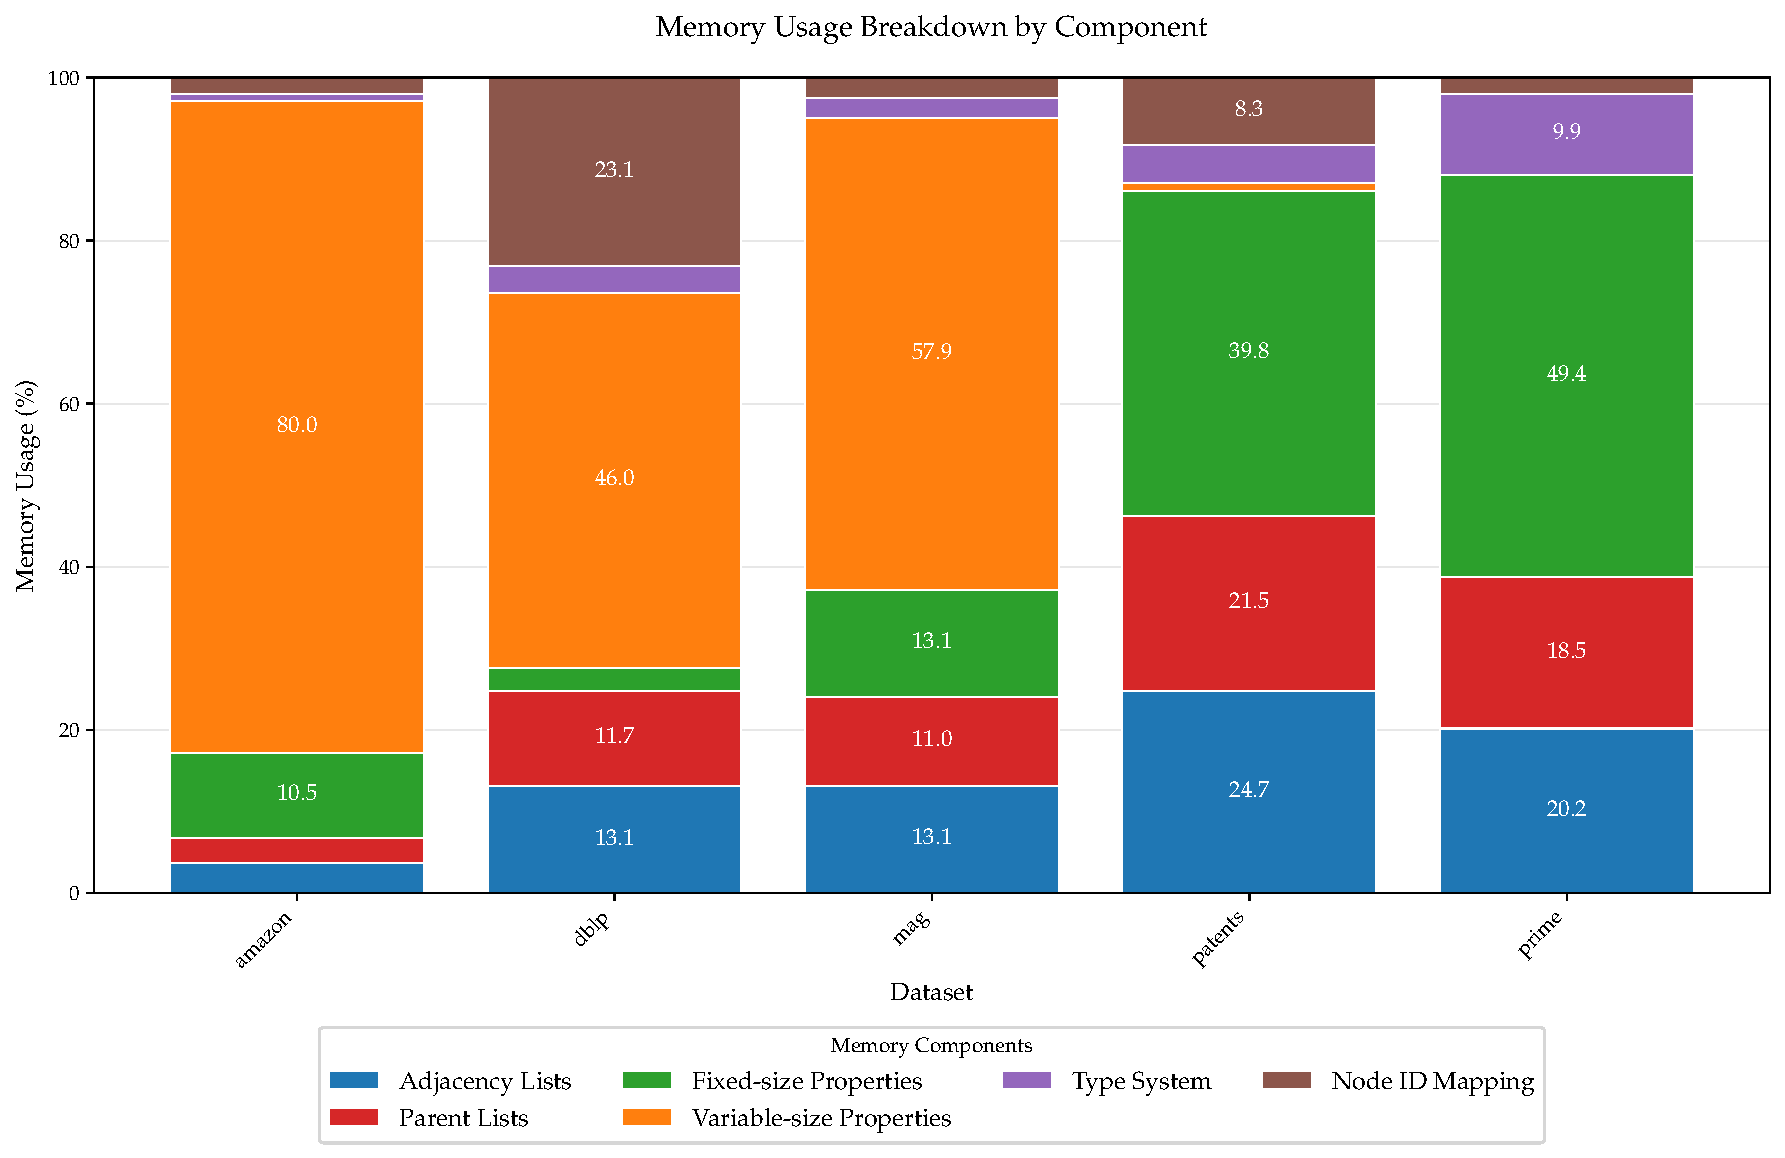
\includegraphics[width=\linewidth]{plots/graph_db_memory_breakdown.pdf}
  \caption{Memory usage breakdown by component in our graph database.}
  \label{fig:space_breakdown}
\end{figure}
\FloatBarrier

These results also support our design discussed in Chapter~\ref{chap:properties}, indicating minimal overhead from our type system. This type system provides the additional benefit of avoiding the storage overhead of null fixed-size properties. For instance, we observed a 70\% reduction in space required for node fixed-size properties in the prime dataset.



As emphasized earlier in Section~\ref{sec:relabelling}, node relabeling plays a crucial role on the compression effectiveness. Figure~\ref{fig:relabelling_effectiveness} highlights such intuition by comparing various relabeling methods, showing that traversal-based strategies consistently outperform default and random node orders. This aligns precisely with our theoretical expectations, given that traversal-based techniques empirically minimize graph bandwidth. Among traversal-based methods, we chose Cuthill-McKee ordering due to its long-standing effectiveness and widespread adoption in practical scenarios. We also evaluated the Degree Minimization heuristic employed in LogGraph, which, however, exhibited moderate-to-high variance in the resulting compression rates.

\begin{figure}[htbp]
  \centering
  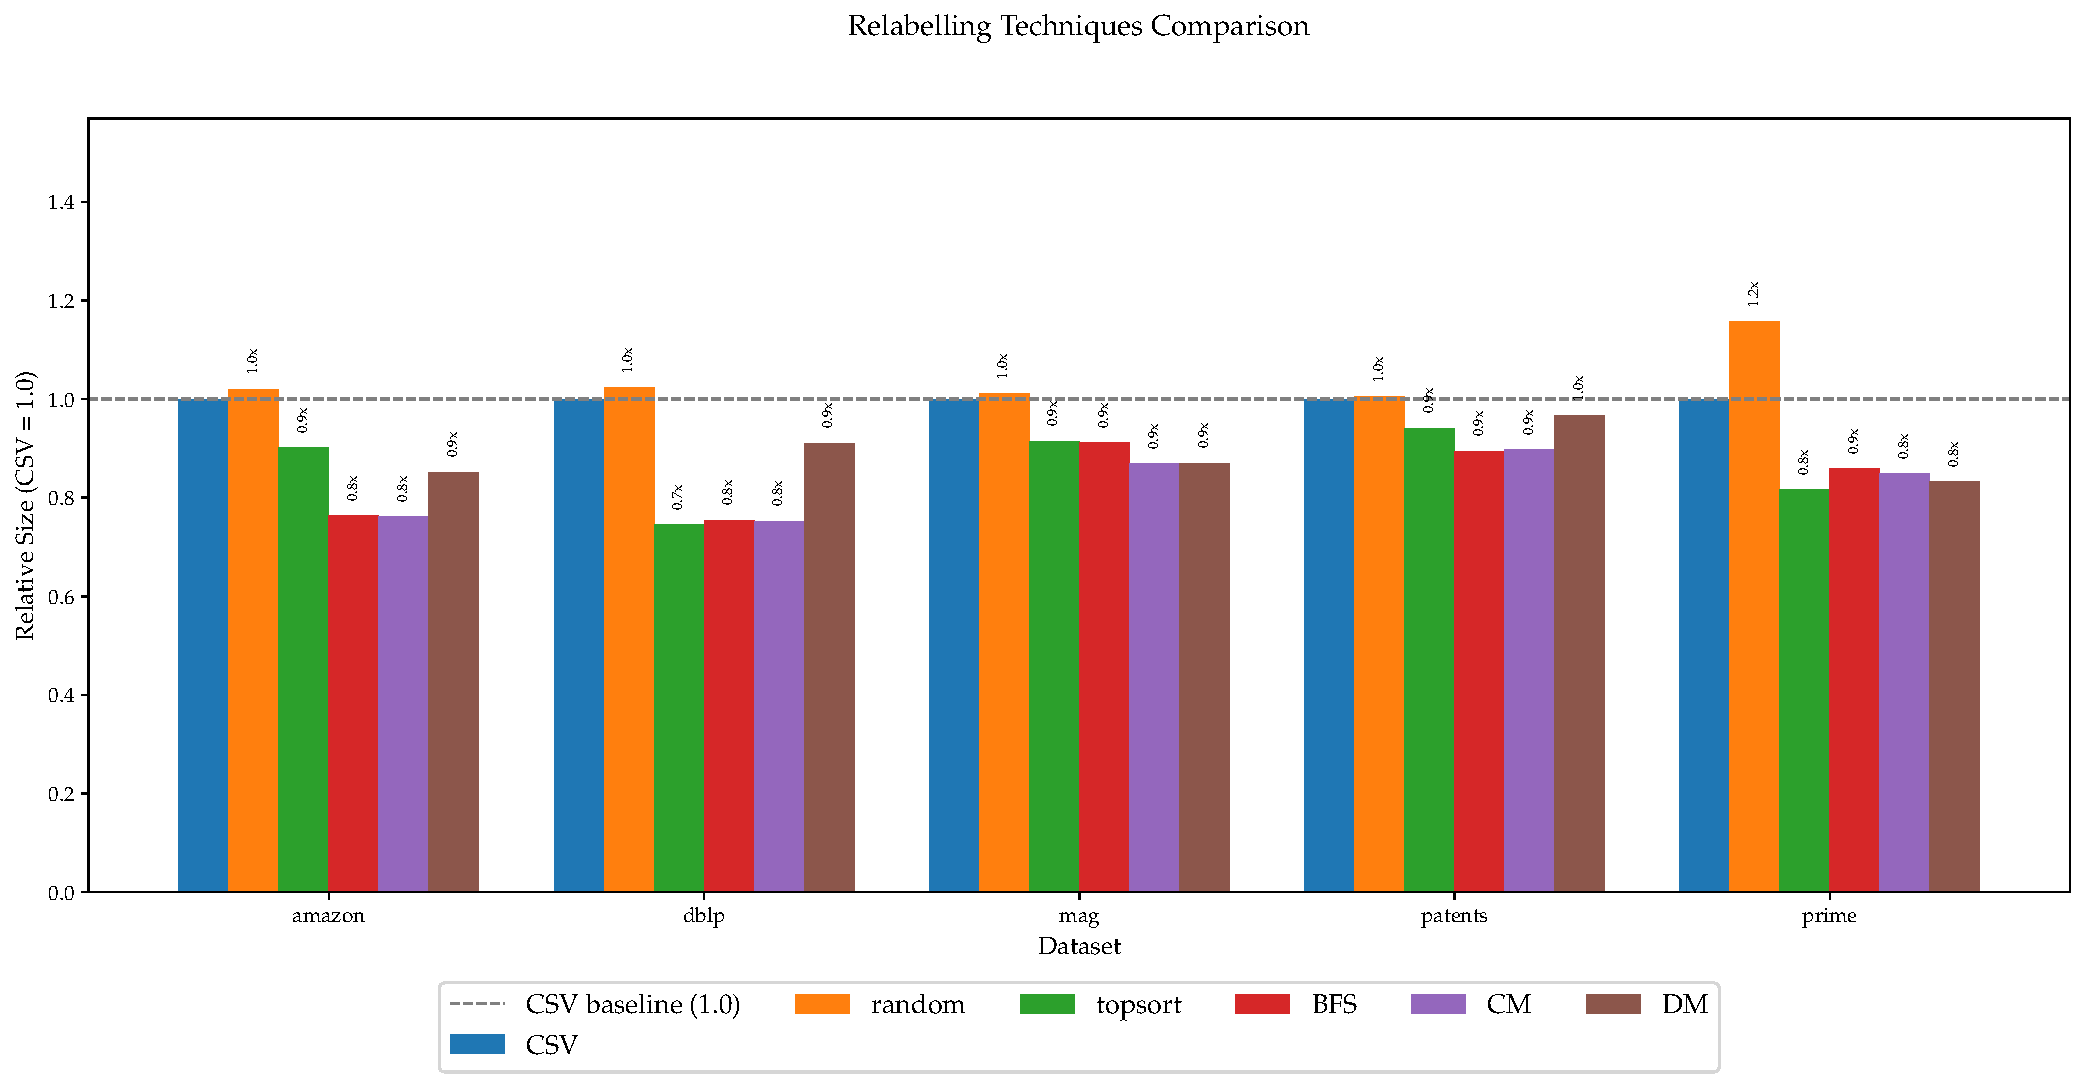
\includegraphics[width=\linewidth]{plots/relabelling.pdf}
  \caption{Impact of relabeling strategies on compression, relative to default CSV order. Note: the topological sort ordering was performed after removing any cycles.}
  \label{fig:relabelling_effectiveness}
\end{figure}
\FloatBarrier

\section{Comparisons with Graph Compressors}

We first evaluate the space and query performance of our adjacency-list representation against existing compressed graph structures (CSR, LogGraph, CGraphIndex). Specifically, Table~\ref{tab:space_usage} and Figure~\ref{fig:adj_size_comparison} show the absolute and relative space required by our GraphDB, LogGraph, and CGraphIndex, compared to the Compressed Sparse Row representation that compresses the offsets with EF and represents the concatenated adjacency lists through bit-packing.

\begin{table}[htbp]
  \centering
  \caption{Storage (in MB) comparison with different graph representations.}
  \label{tab:space_usage}
  \begin{tabular}{lrrrr}
    \toprule
    Dataset & CSR & LogGraph & CGraphIndex & Our Approach \\
    \midrule
    amazon  &  20.1 &  17.0 &  28.6 & \textbf{13.7} \\
    dblp    & 218.2 & 214.7 & 411.2 & \textbf{156.7} \\
    mag     & 102.7 &  \textbf{76.4} & 107.6 &  79.5 \\
    patents & 143.3 & 137.6 & 171.7 & \textbf{124.6} \\
    prime   &  16.7 &   \textbf{9.5} &  15.0 &  9.6 \\
    \bottomrule
  \end{tabular}
\end{table}
\FloatBarrier

Our approach achieves the highest compactness on sparse graphs, clearly outperforming CGraphIndex and LogGraph, both of which exhibit notable inefficiencies when representing such graphs. On denser, more connected graphs, our method still delivers compelling compression ratios, comparable to or better than LogGraph, which ranks second in this benchmark.

\begin{figure}[htbp]
  \centering
  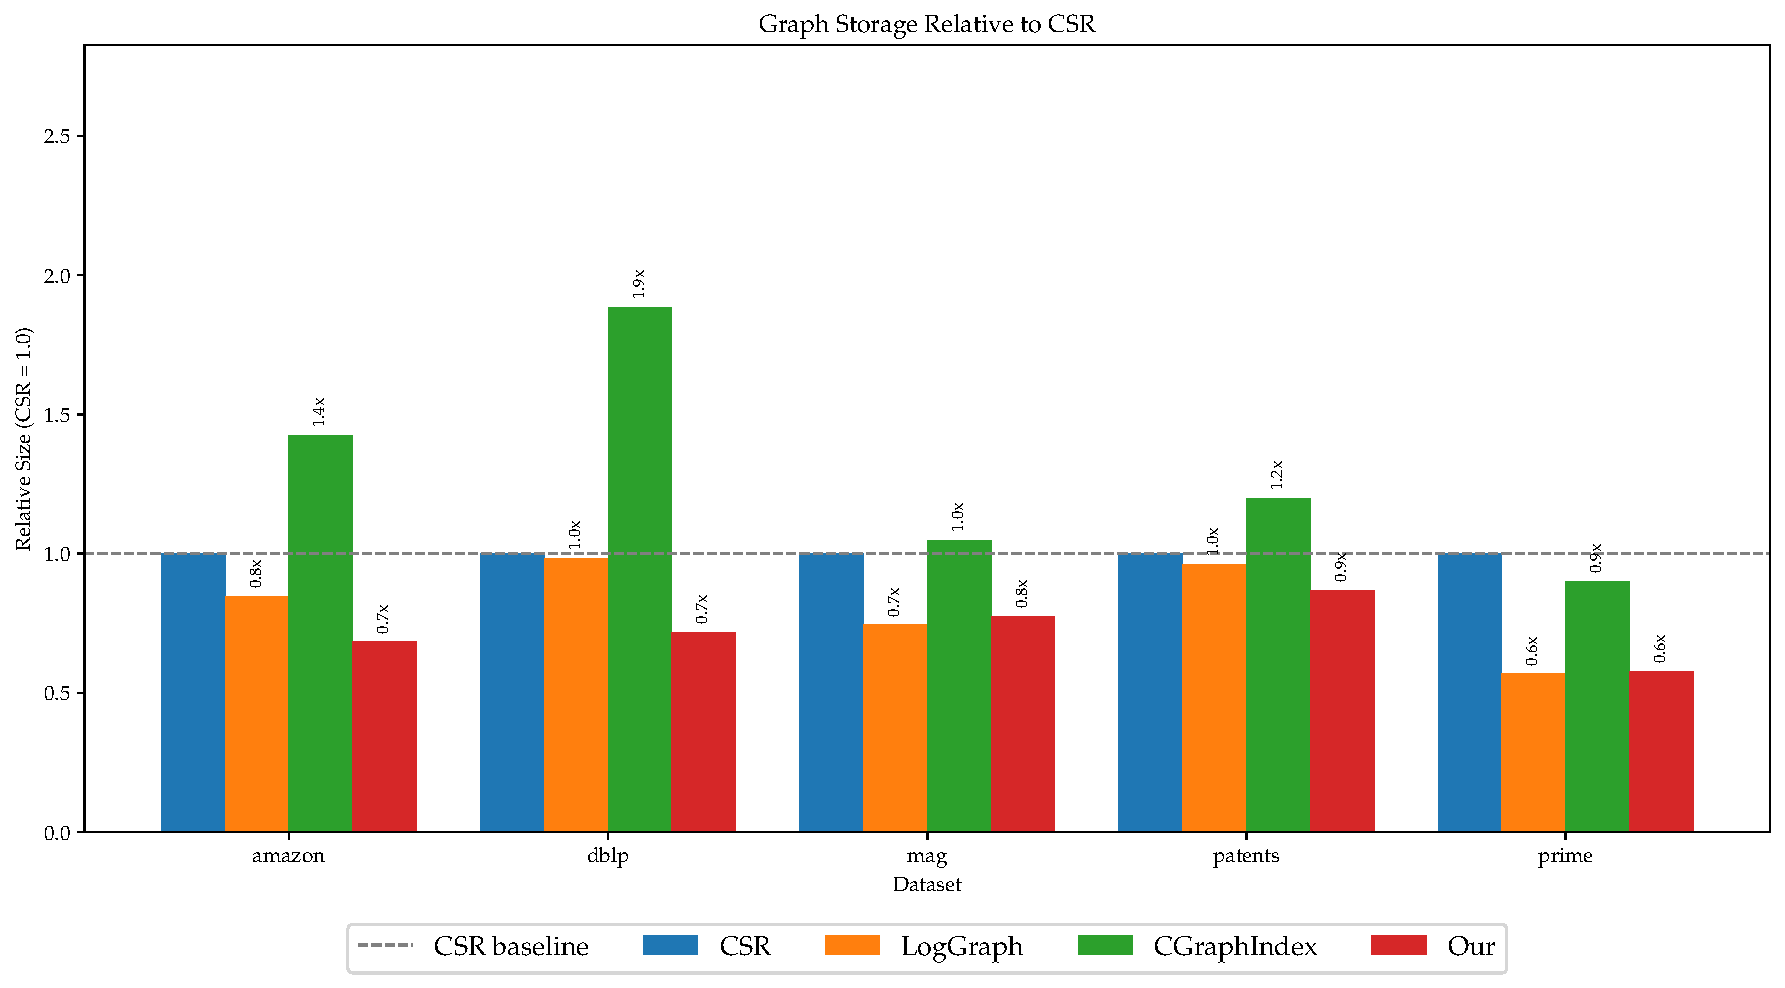
\includegraphics[width=\linewidth]{plots/adj_size_comparison.pdf}
  \caption{Adjacency-list storage sizes normalized to CSR, including our approach.}
  \label{fig:adj_size_comparison}
\end{figure}
\FloatBarrier

Similarly, Table~\ref{tab:adj_time_usage_neighbors} and Figure~\ref{fig:adj_time_comparison} show the absolute and relative performance results for single-hop neighbor-query retrieval compared to other compressed graph representations.

\begin{table}[htbp]
\centering
\caption{Average single-hop neighbor query times (ns per neighbor).}
\label{tab:adj_time_usage_neighbors}
\begin{tabular}{lrrrr}
\toprule
Dataset & CSR & LogGraph & CGraphIndex & Our Approach \\
\midrule
amazon  & \textbf{30.51} & 270.70 &  38.08 &  38.14 \\
dblp    &  61.52 & 602.90 &   \textbf{6.34} & 122.91 \\
mag     & \textbf{16.51} &  82.87 &  23.24 &  31.90 \\
patents &  23.64 & 121.76 &   \textbf{3.77} &  43.65 \\
prime   &  \textbf{4.23} &  17.10 &   5.98 &   9.26 \\
\bottomrule
\end{tabular}
\end{table}
\FloatBarrier

The results show that CSR performs best on dense graphs, whereas CGraphIndex achieves better performance on datasets such as $\verb^patents^$ and $\verb^dblp^$. Our approach consistently achieves execution times typically less than twice that of CSR. Additionally, it greatly outperforms LogGraph on all tested datasets and provides speeds comparable to CGraphIndex on datasets such as $\verb^amazon^$ and $\verb^mag^$.

\begin{figure}[htbp]
  \centering
  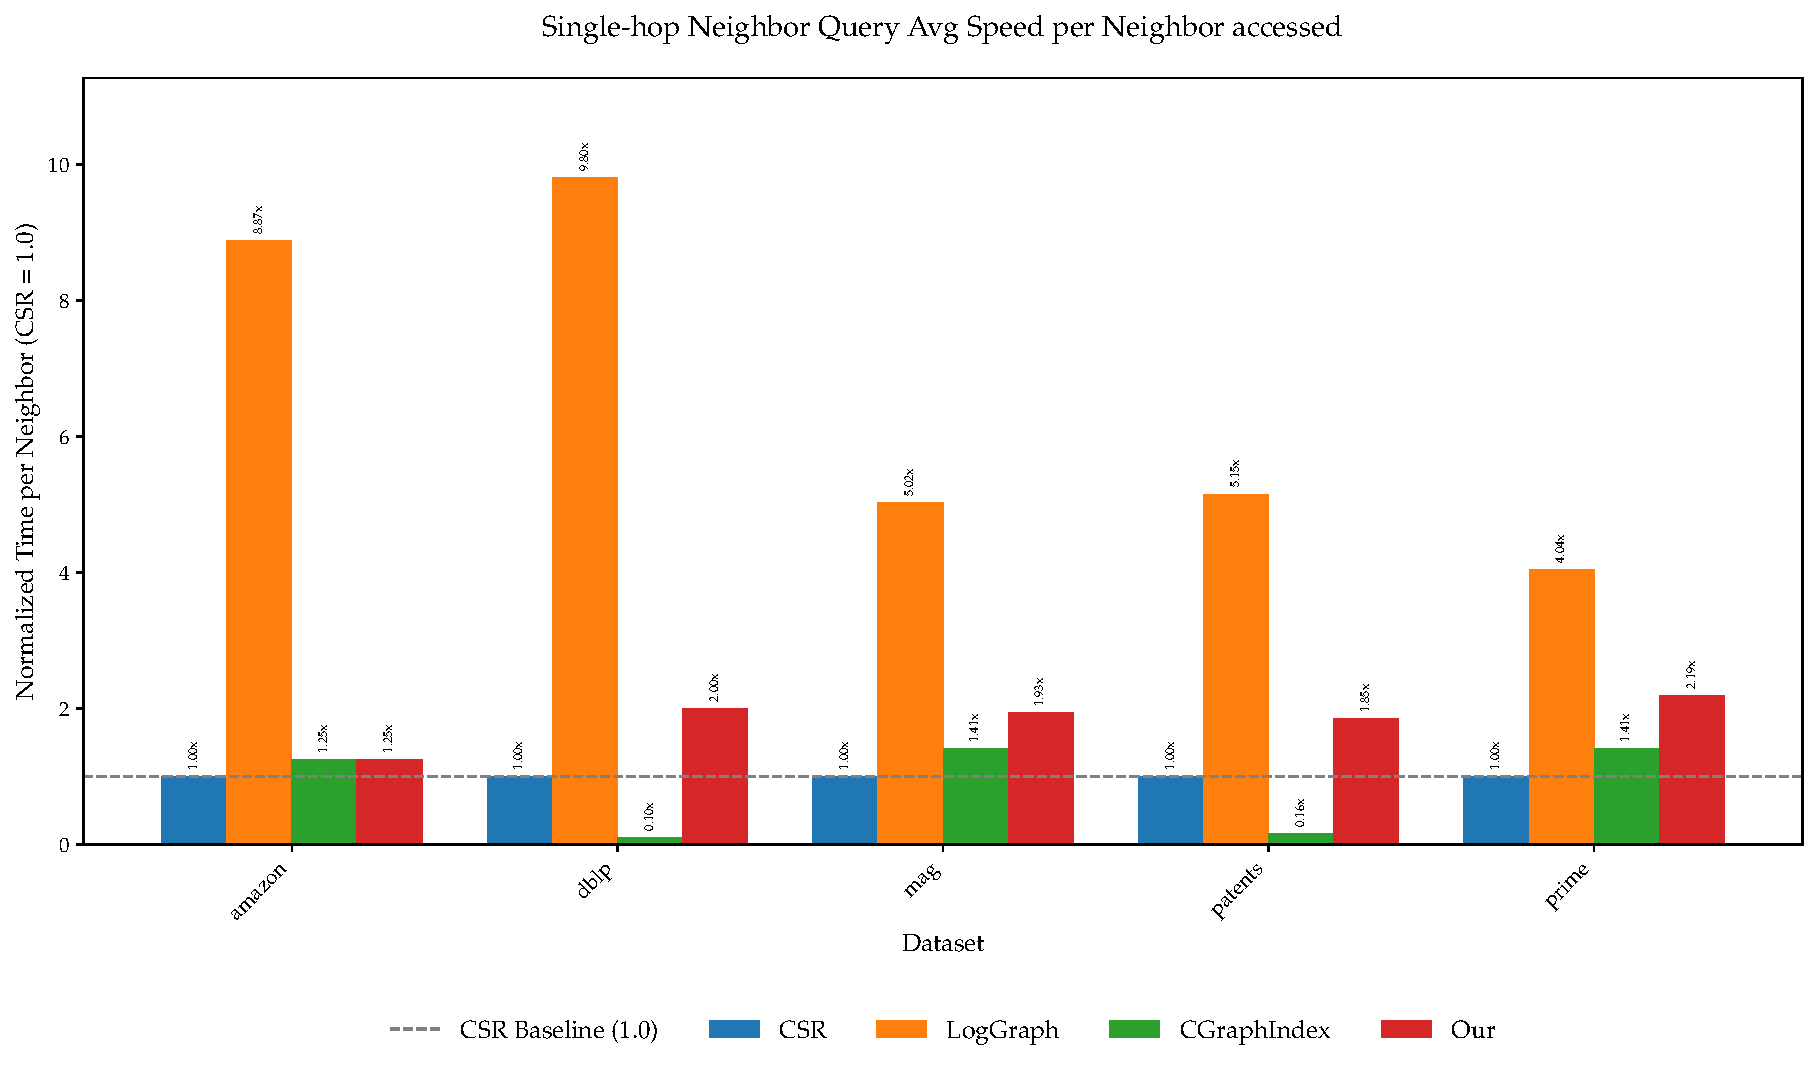
\includegraphics[width=\linewidth]{plots/adj_neighbors_comparison.pdf}
  \caption{Single-hop neighbor query performance comparison between compressed graph representations.}
  \label{fig:adj_time_comparison}
\end{figure}
\FloatBarrier

The Pareto-frontier analysis presented in Figure~\ref{fig:pareto_frontiers}, incorporating the discussed results, confirms that both CSR and our approach consistently achieve competitive, and occasionally superior, space-time trade-offs compared to the other approaches. In fact, the benchmarking clearly positions our method along the Pareto frontier regarding trade-offs between space consumption and query time across all examined datasets. In contrast, CGraphIndex and LogGraph do not consistently appear on the Pareto frontier, indicating that their space-time efficiency is less uniform across different datasets.

\begin{figure}[htbp]
  \centering
  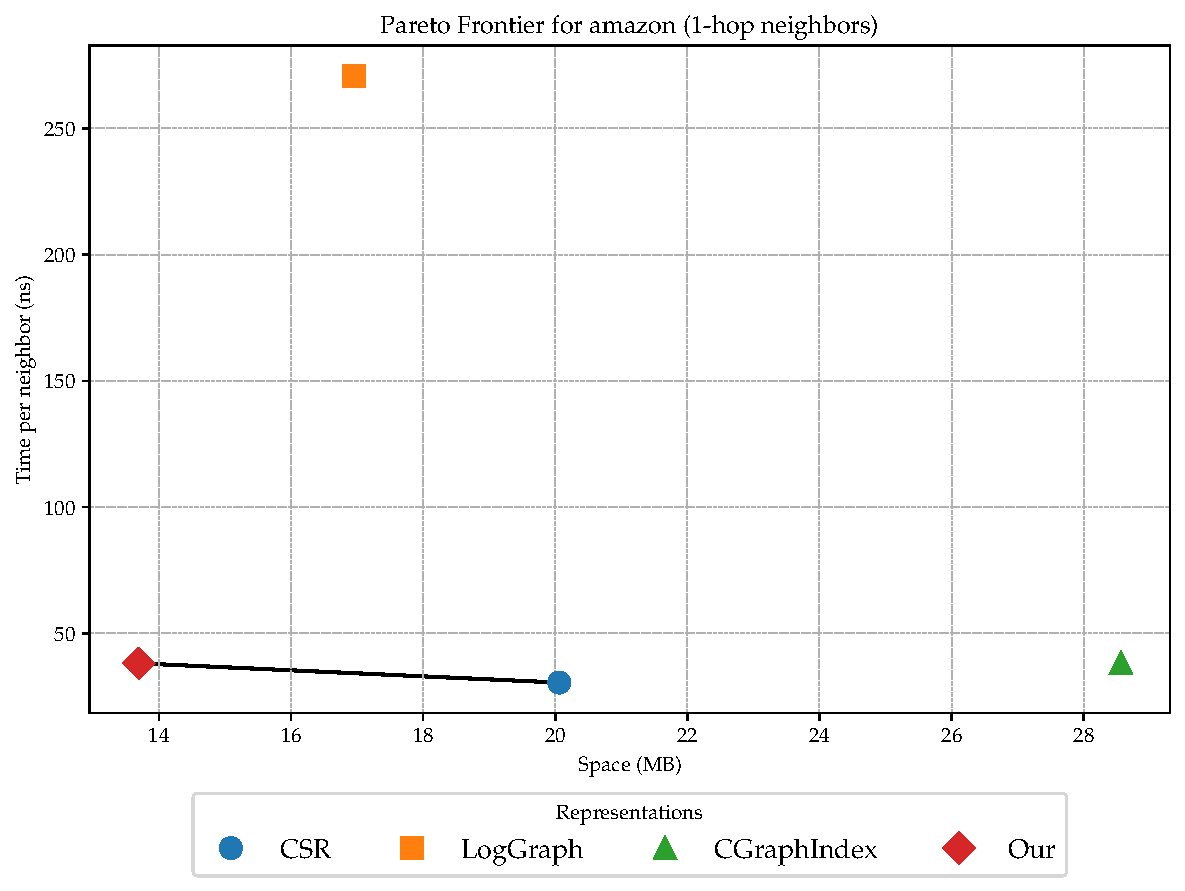
\includegraphics[width=0.45\linewidth]{plots/neighbors/amazon.pdf}\hfill
  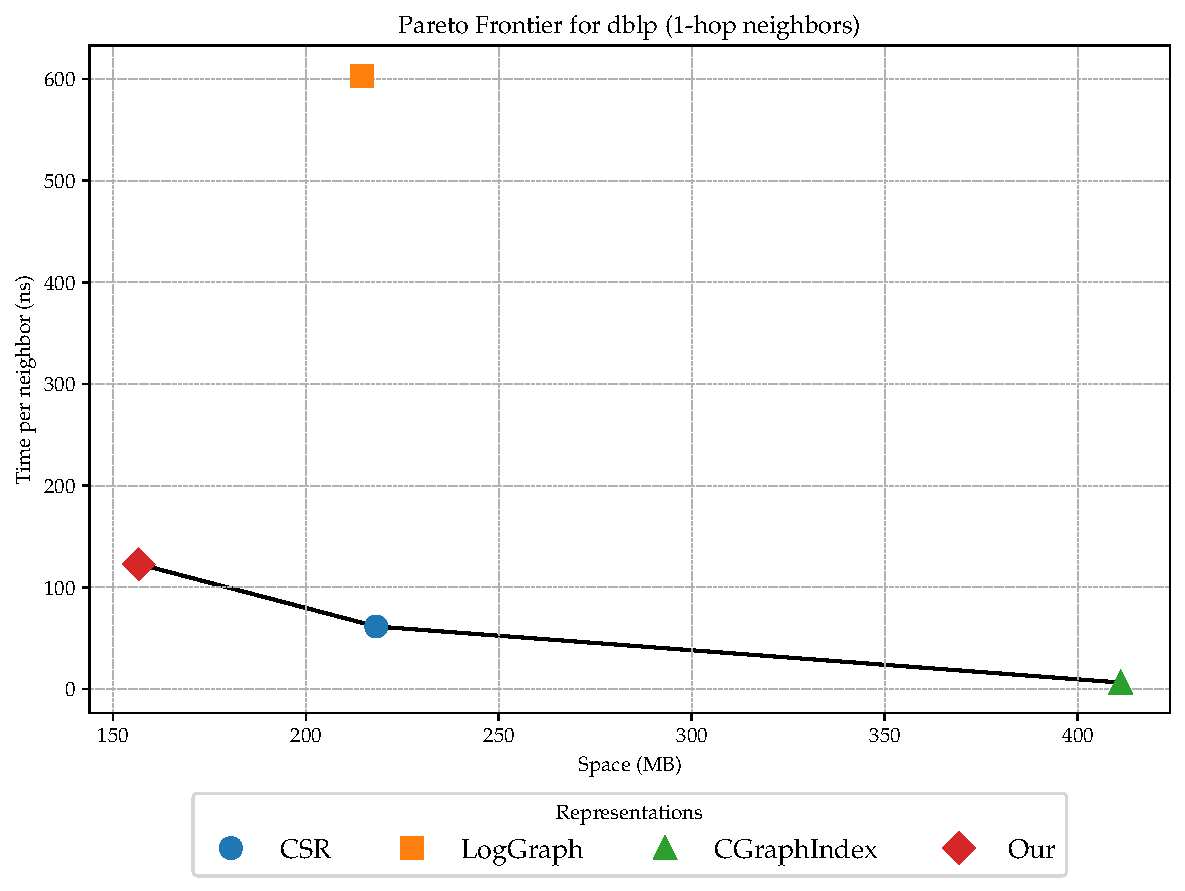
\includegraphics[width=0.45\linewidth]{plots/neighbors/dblp.pdf}
  
  \vspace{1em}
  
  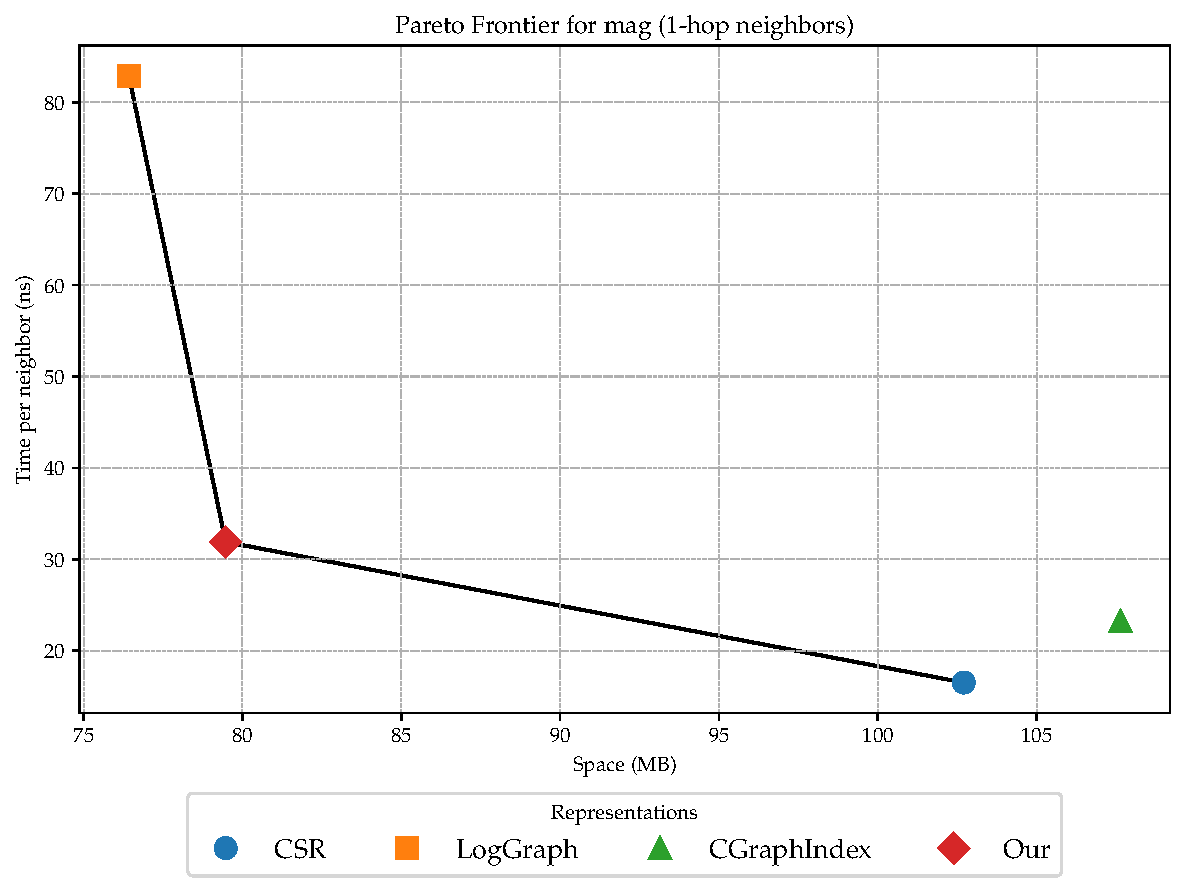
\includegraphics[width=0.45\linewidth]{plots/neighbors/mag.pdf}\hfill
  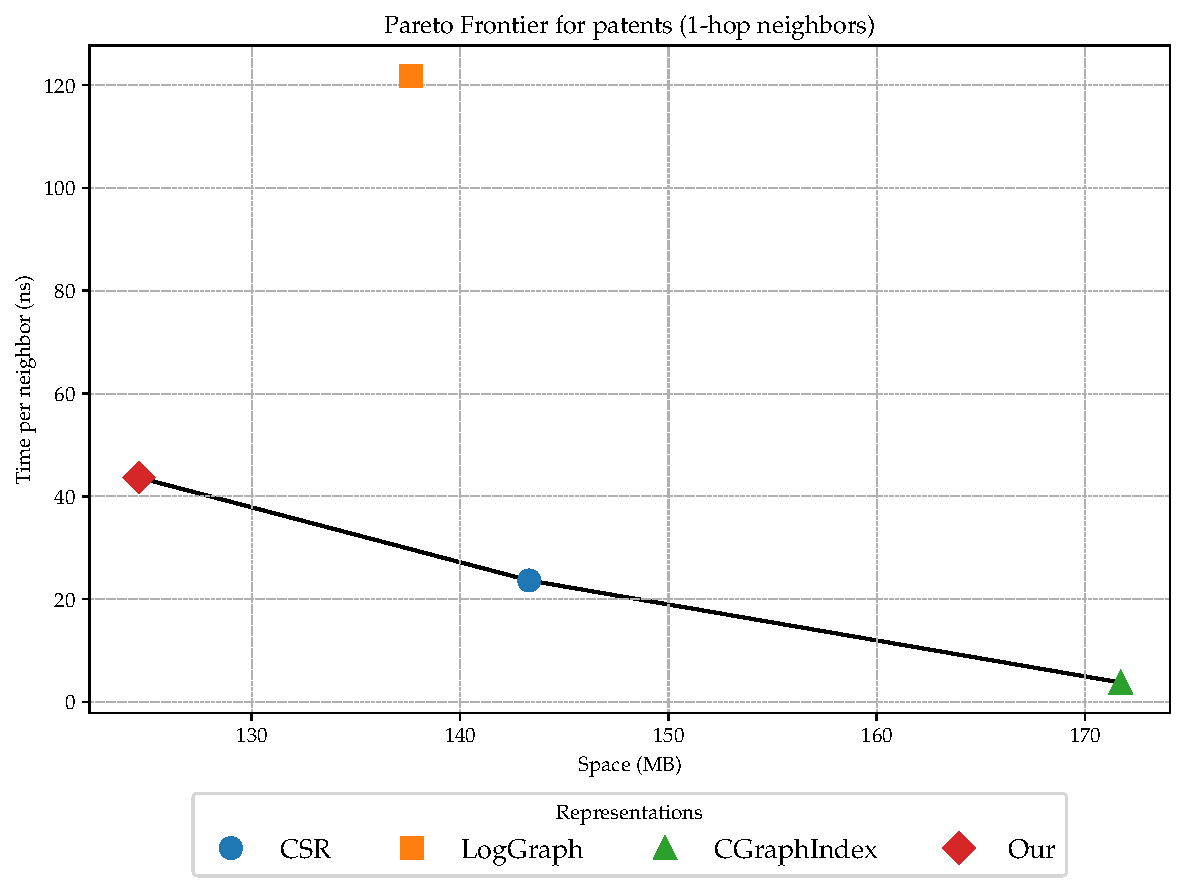
\includegraphics[width=0.45\linewidth]{plots/neighbors/patents.pdf}
  
  \vspace{1em}
  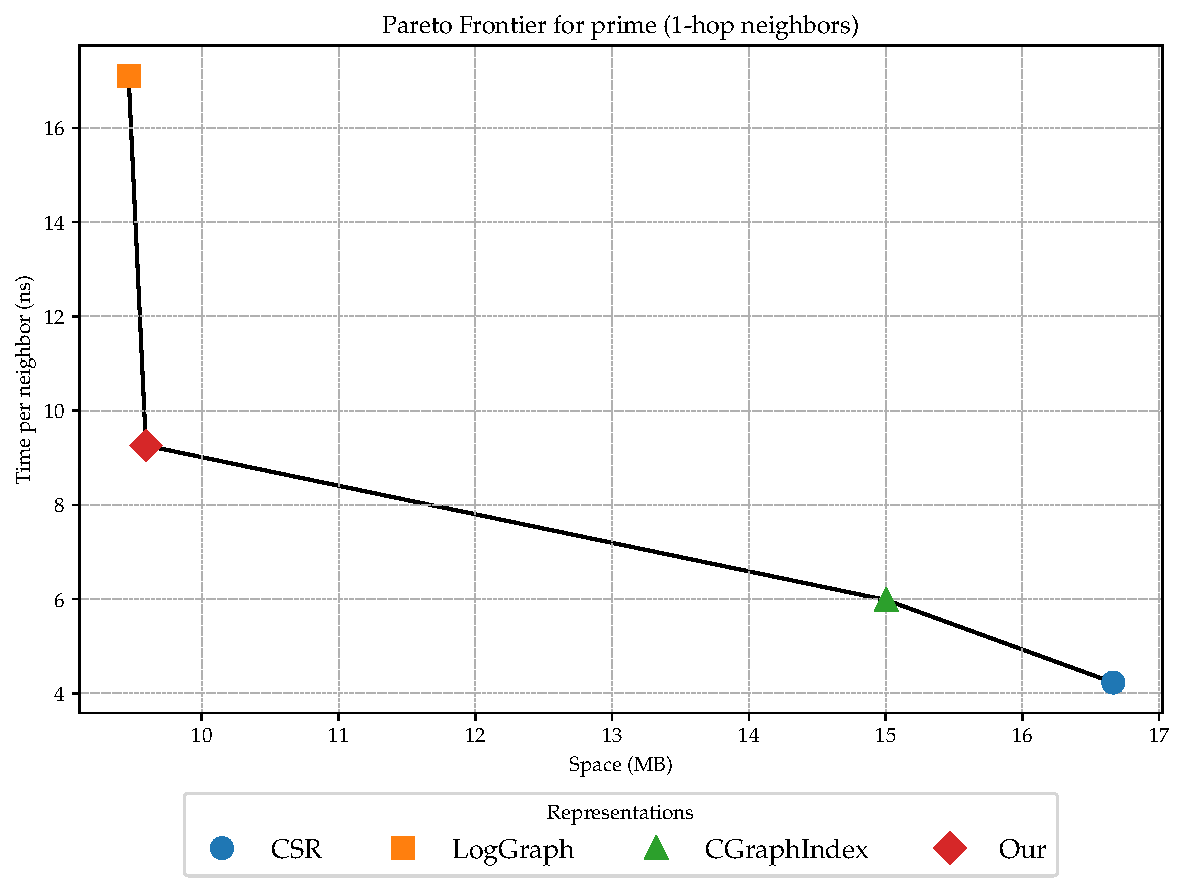
\includegraphics[width=0.45\linewidth]{plots/neighbors/prime.pdf}
  \caption{Pareto frontier analysis for single-hop neighbor queries showing space-time trade-offs across all datasets.}
  \label{fig:pareto_frontiers}
\end{figure}
\FloatBarrier

Regarding two-hop neighborhood queries (Figure~\ref{fig:two_hop_queries}), we observe that LogGraph surprisingly ranks best in some datasets. However, this seemingly superior performance arises because LogGraph treats edges as undirected and thus retrieves both neighbors and parent nodes for each query node. Consequently, LogGraph queries inherently explore the squared number of nodes on average, yet perform an equivalent number of memory operations compared to directed traversal. This behavior disproportionately benefits LogGraph due to normalization effects, resulting in an unfair comparison.

We also note that CGraphIndex generally achieves better performance than CSR and our method, particularly on sparse graphs. For completeness, we tested an uncompressed CSR variant as well, but noted only marginal improvements. Therefore, we attribute the observed performance gap primarily to implementation specifics rather than fundamental design advantages. We are confident that such specific implementation choices could be equivalently incorporated into both CSR and our method.

\begin{figure}[htbp]
  \centering
  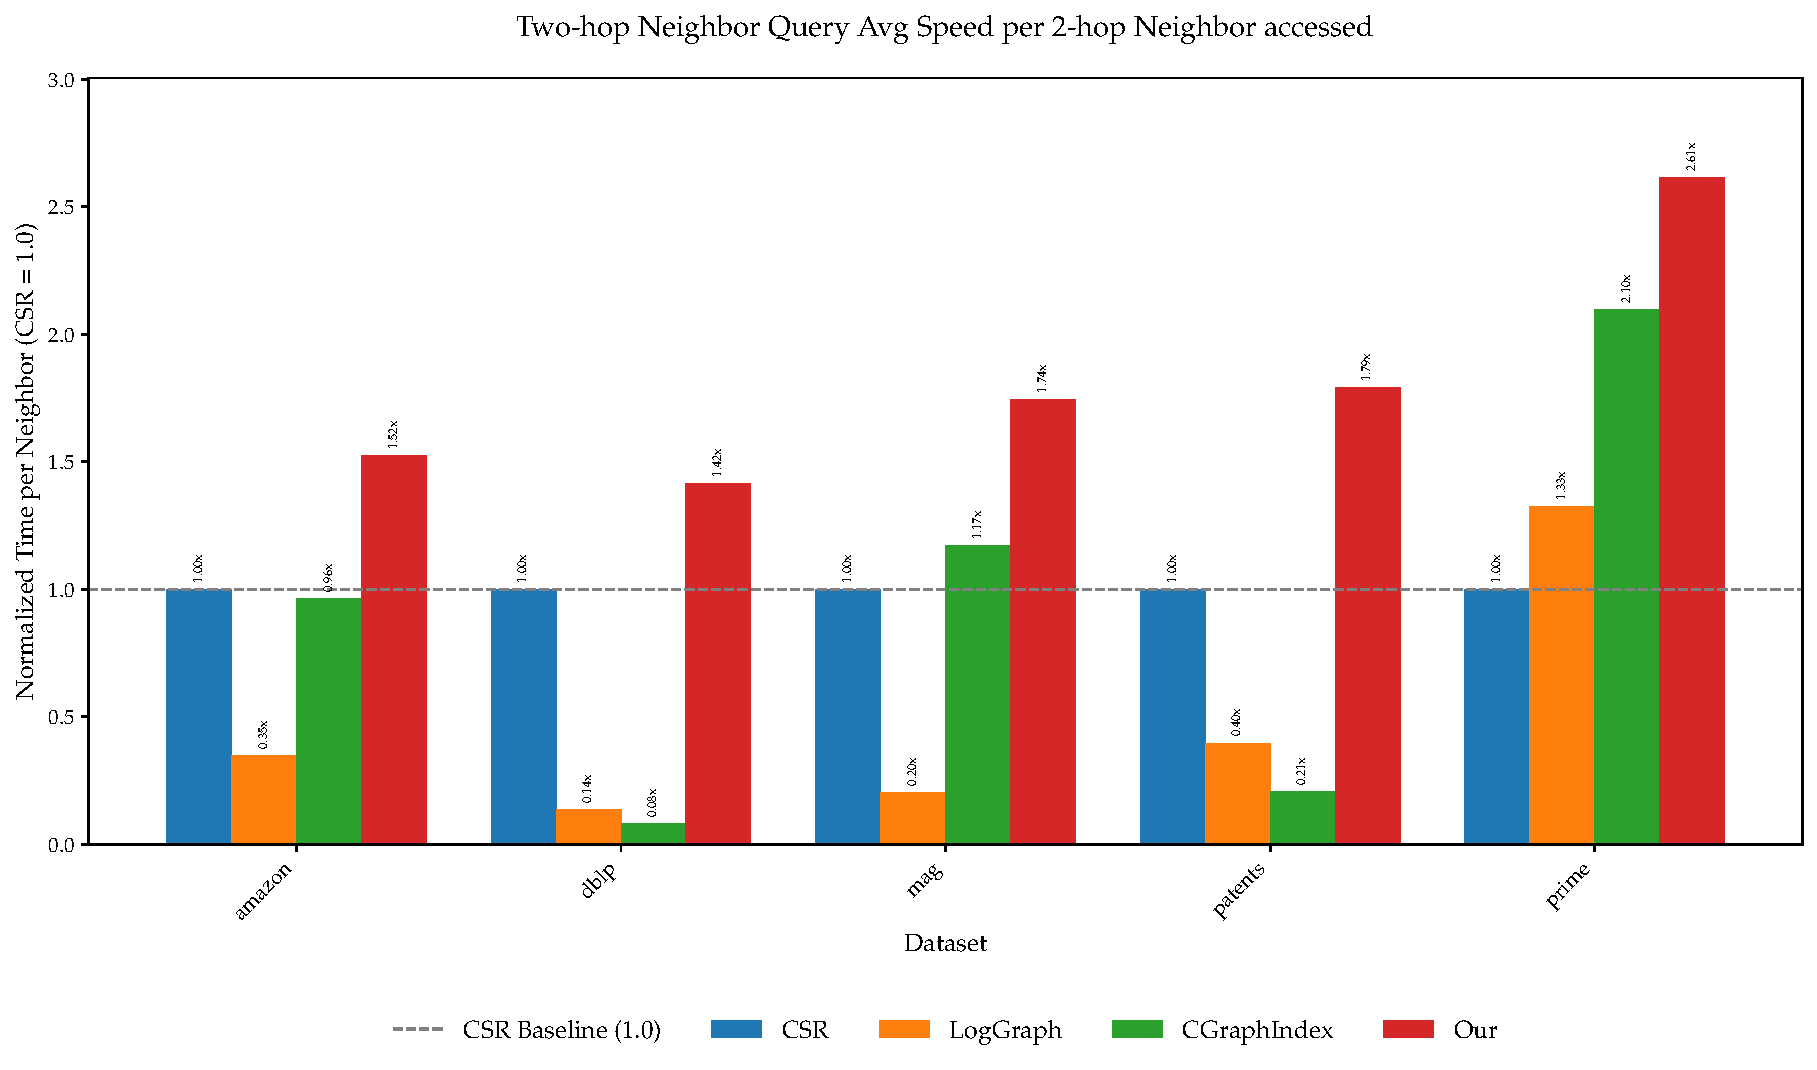
\includegraphics[width=\linewidth]{plots/adj_2neighbors_comparison.pdf}
  \caption{Two-hop neighbor query performance comparison between compressed graph representations.}
  \label{fig:two_hop_queries}
\end{figure}
\FloatBarrier

Finally, we highlight that our approach demonstrates strong versatility, effectively accommodating either scenario—whether storage space efficiency or query-time speed is the more critical priority. On the one hand, our method significantly reduces space usage compared to conventional representations, making it an ideal choice in situations where minimizing memory footprint is paramount. On the other hand, our representation can smoothly adapt towards faster decompression by setting \( h=0 \), thus matching the CSR benchmark's performance in settings that prioritize query speed.

\section{Comparison with Graph Databases}

We now compare storage usage and query times against Neo4j and ArangoDB. Following recent literature, we primarily compare to Neo4j as it outperforms ArangoDB in graph processing tasks~\cite{sandell2024}. All experiments on Neo4j use batched queries for improved performance.

In terms of storage usage, our approach substantially outperforms both Neo4j and ArangoDB, achieving database sizes that are also significantly smaller than zipped versions of the original datasets, as shown in Figure~\ref{fig:storage_vs_files} and Table~\ref{tab:gdb_space_usage}

\begin{figure}[htbp]
  \centering
  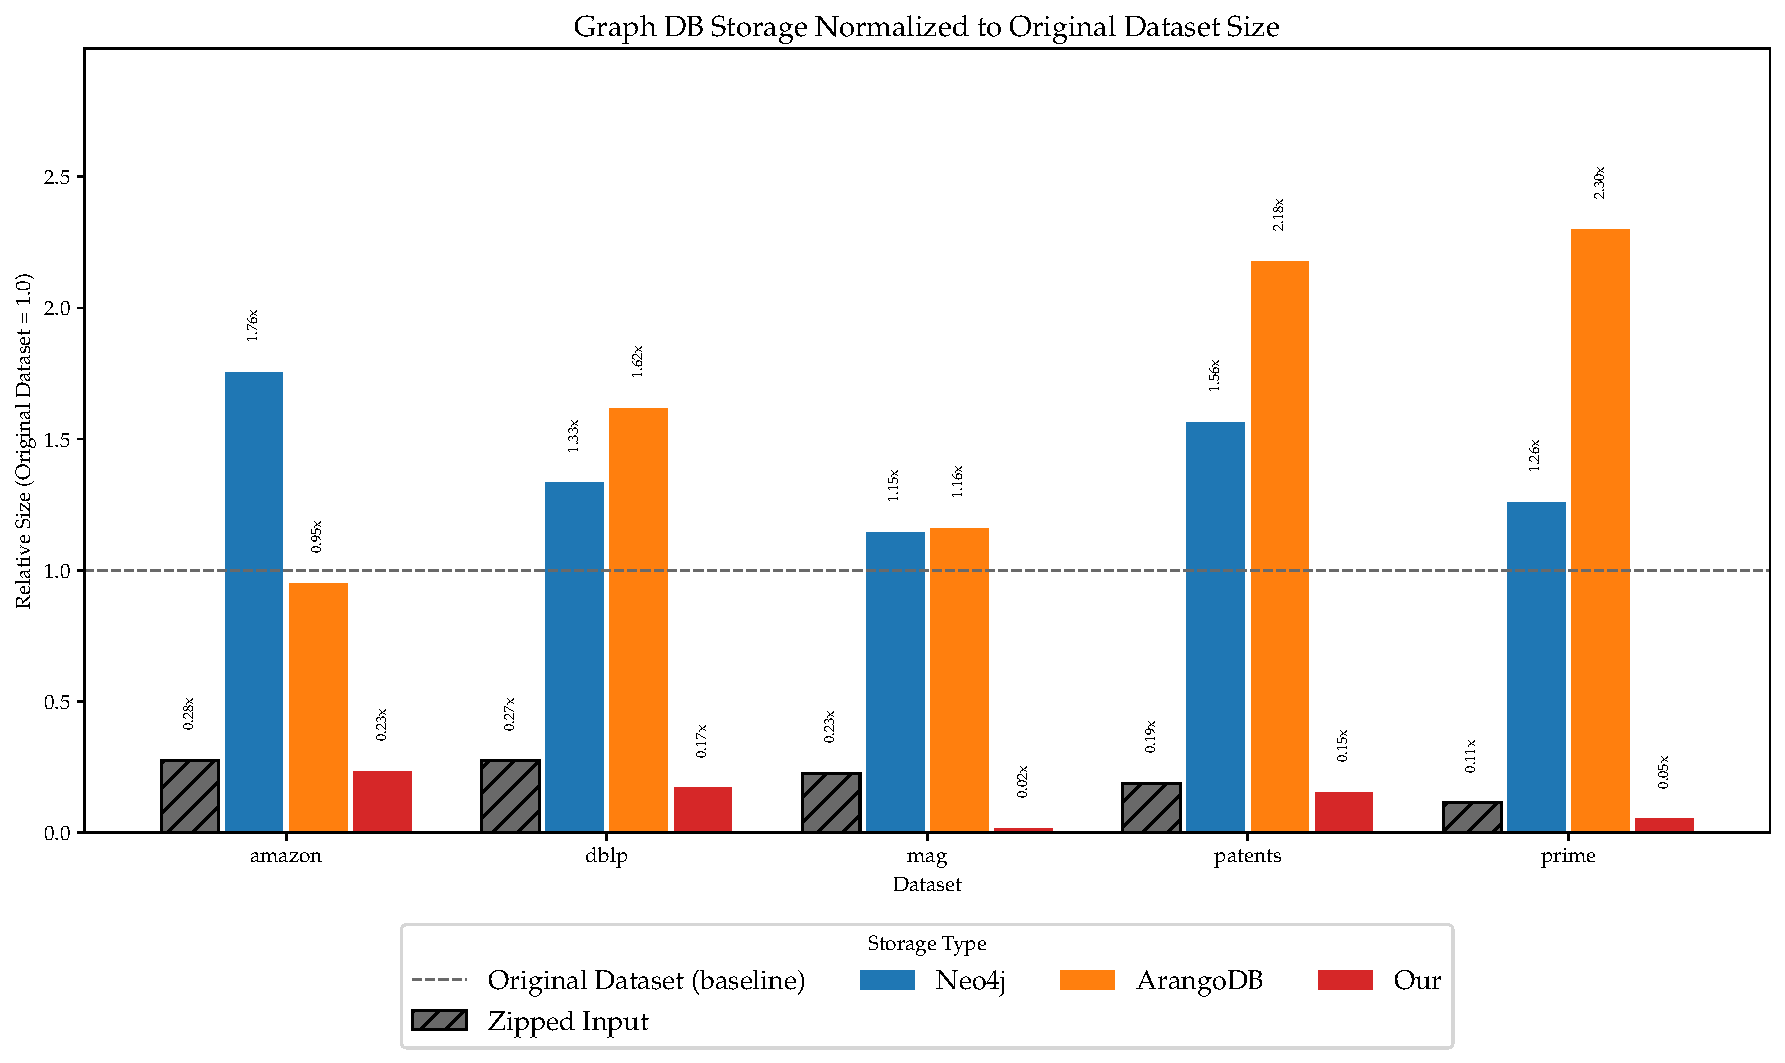
\includegraphics[width=\linewidth]{plots/graphdb_storage.pdf}
  \caption{Database size comparison normalized against original datasets.}
  \label{fig:storage_vs_files}
\end{figure}
\FloatBarrier

\begin{table}[htbp]
  \centering
  \caption{Database sizes (MB) for different storage options and systems.}
  \label{tab:gdb_space_usage}
  \resizebox{\textwidth}{!}{%
    \begin{tabular}{lrrrrr}
      \toprule
      Dataset & Zipped data & Unzipped data & ArangoDB & Neo4j & Our Approach \\
      \midrule
      amazon   & 208.8  & 758.3  & 721.2  & 1331.2 & \textbf{177.7} \\
      dblp     & 903.1  & 3301.1 & 5336.7 & 4403.2 & \textbf{563.9} \\
      mag      & 388.9  & 1716.4 & 1991.1 & 1965.7 & \textbf{27.5}  \\
      patents  & 233.9  & 1244.4 & 2709.1 & 1945.6 & \textbf{192.6} \\
      prime    &  28.3  &  248.0 &  570.0 &  312.0 & \textbf{13.1}  \\
      \bottomrule
    \end{tabular}
  }
\end{table}
\FloatBarrier

Our solution also significantly surpasses Neo4j in performance for both single-hop and two-hop neighbor queries, as shown in Tables \ref{tab:gdb_neighbors_time} and \ref{tab:gdb_neighbors2_time}.

\begin{table}[htbp]
  \centering
  \begin{minipage}{0.48\textwidth}
\centering
\caption{Single-hop neighbor query times (ns per neighbor).}
\label{tab:gdb_neighbors_time}
\begin{tabular}{lrr}
\toprule
Dataset & Neo4j & Our Approach \\
\midrule
amazon   & 210.8   & \textbf{38.14}  \\
dblp     & 1250.3  & \textbf{122.91} \\
mag      & 180.7   & \textbf{31.90}  \\
patents  & 320.1   & \textbf{43.65}  \\
prime    & 45.2    & \textbf{9.26}   \\
\bottomrule
\end{tabular}
\end{minipage}
  \hfill
\begin{minipage}{0.48\textwidth}
\centering
\caption{Two-hop neighbor query times (ns per neighbor).}
\label{tab:gdb_neighbors2_time}
\begin{tabular}{lrr}
\toprule
Dataset & Neo4j & Our Approach \\
\midrule
amazon   & 450.2   & \textbf{10.48}  \\
dblp     & 2850.7  & \textbf{118.93} \\
mag      & 420.3   & \textbf{18.81}  \\
patents  & 680.9   & \textbf{38.83}  \\
prime    & 95.4    & \textbf{4.73}   \\
\bottomrule
\end{tabular}
\end{minipage}
\end{table}
\FloatBarrier

While we also achieve faster fixed-size property retrievals (Table \ref{tab:gdb_fixed_props_time}), our variable-size property retrievals are comparatively slower (Table \ref{tab:gdb_var_props_time}). This reflects an intentional trade-off: highly compressed FM-index encoding significantly saves space for infrequently accessed data, at a known performance cost. These parameters could be relaxed to favor faster retrieval if needed.

\begin{table}[htbp]
  \centering
  \begin{minipage}{0.48\textwidth}
    \centering
    \caption{Fixed-size property throughput (MB/s).}
    \label{tab:gdb_fixed_props_time}
    \begin{tabular}{lrr}
      \toprule
      Dataset & Neo4j & Our Approach \\
      \midrule
      amazon   & 1.8  & \textbf{27.3} \\
      dblp     & 1.5  & \textbf{25.2} \\
      mag      & 2.0  & \textbf{35.5} \\
      patents  & 1.5  & \textbf{38.8} \\
      prime    & 1.7  & \textbf{38.3} \\
      \bottomrule
    \end{tabular}
  \end{minipage}
  \hfill
  \begin{minipage}{0.48\textwidth}
    \centering
    \caption{Variable-size property throughput (KB/s).}
    \label{tab:gdb_var_props_time}
    \begin{tabular}{lrr}
      \toprule
      Dataset & Neo4j & Our Approach \\
      \midrule
      amazon   & \textbf{1154.9}   & 7.6 \\
      dblp     & \textbf{5810.0}  & 29.4 \\
      mag      & \textbf{4942.5}  & 21.7 \\
      patents  & \textbf{870.7}  & 13.5 \\
      \bottomrule
    \end{tabular}
  \end{minipage}
\end{table}
\FloatBarrier

In summary, our compressed approach delivers strong benefits in terms of both space efficiency and query speed for frequently executed graph operations, making it particularly attractive in settings where storage constraints exist and variable-sized properties are rarely accessed.
